\documentclass[12pt,a4paper]{article}

\usepackage[utf8]{inputenc}
\usepackage[T2A]{fontenc}
\usepackage{amssymb,amsmath,mathrsfs,amsthm}
\usepackage[russian]{babel}
\usepackage{graphicx}
\usepackage{float}
\usepackage{multirow}
\usepackage[footnotesize]{caption2}
\usepackage{indentfirst}
%\usepackage[ruled,section]{algorithm}
%\usepackage[noend]{algorithmic}
%\usepackage[all]{xy}

% Параметры страницы
\textheight=24cm
\textwidth=16cm
\oddsidemargin=5mm
\evensidemargin=-5mm
\marginparwidth=36pt
\topmargin=-1cm
\footnotesep=3ex
%\flushbottom
\raggedbottom
\tolerance 3000
% подавить эффект "висячих стpок"
\clubpenalty=10000
\widowpenalty=10000
\renewcommand{\baselinestretch}{1.1}
\renewcommand{\baselinestretch}{1.5} %для печати с большим интервалом

\begin{document}

\begin{titlepage}
\begin{center}

    \bigskip
    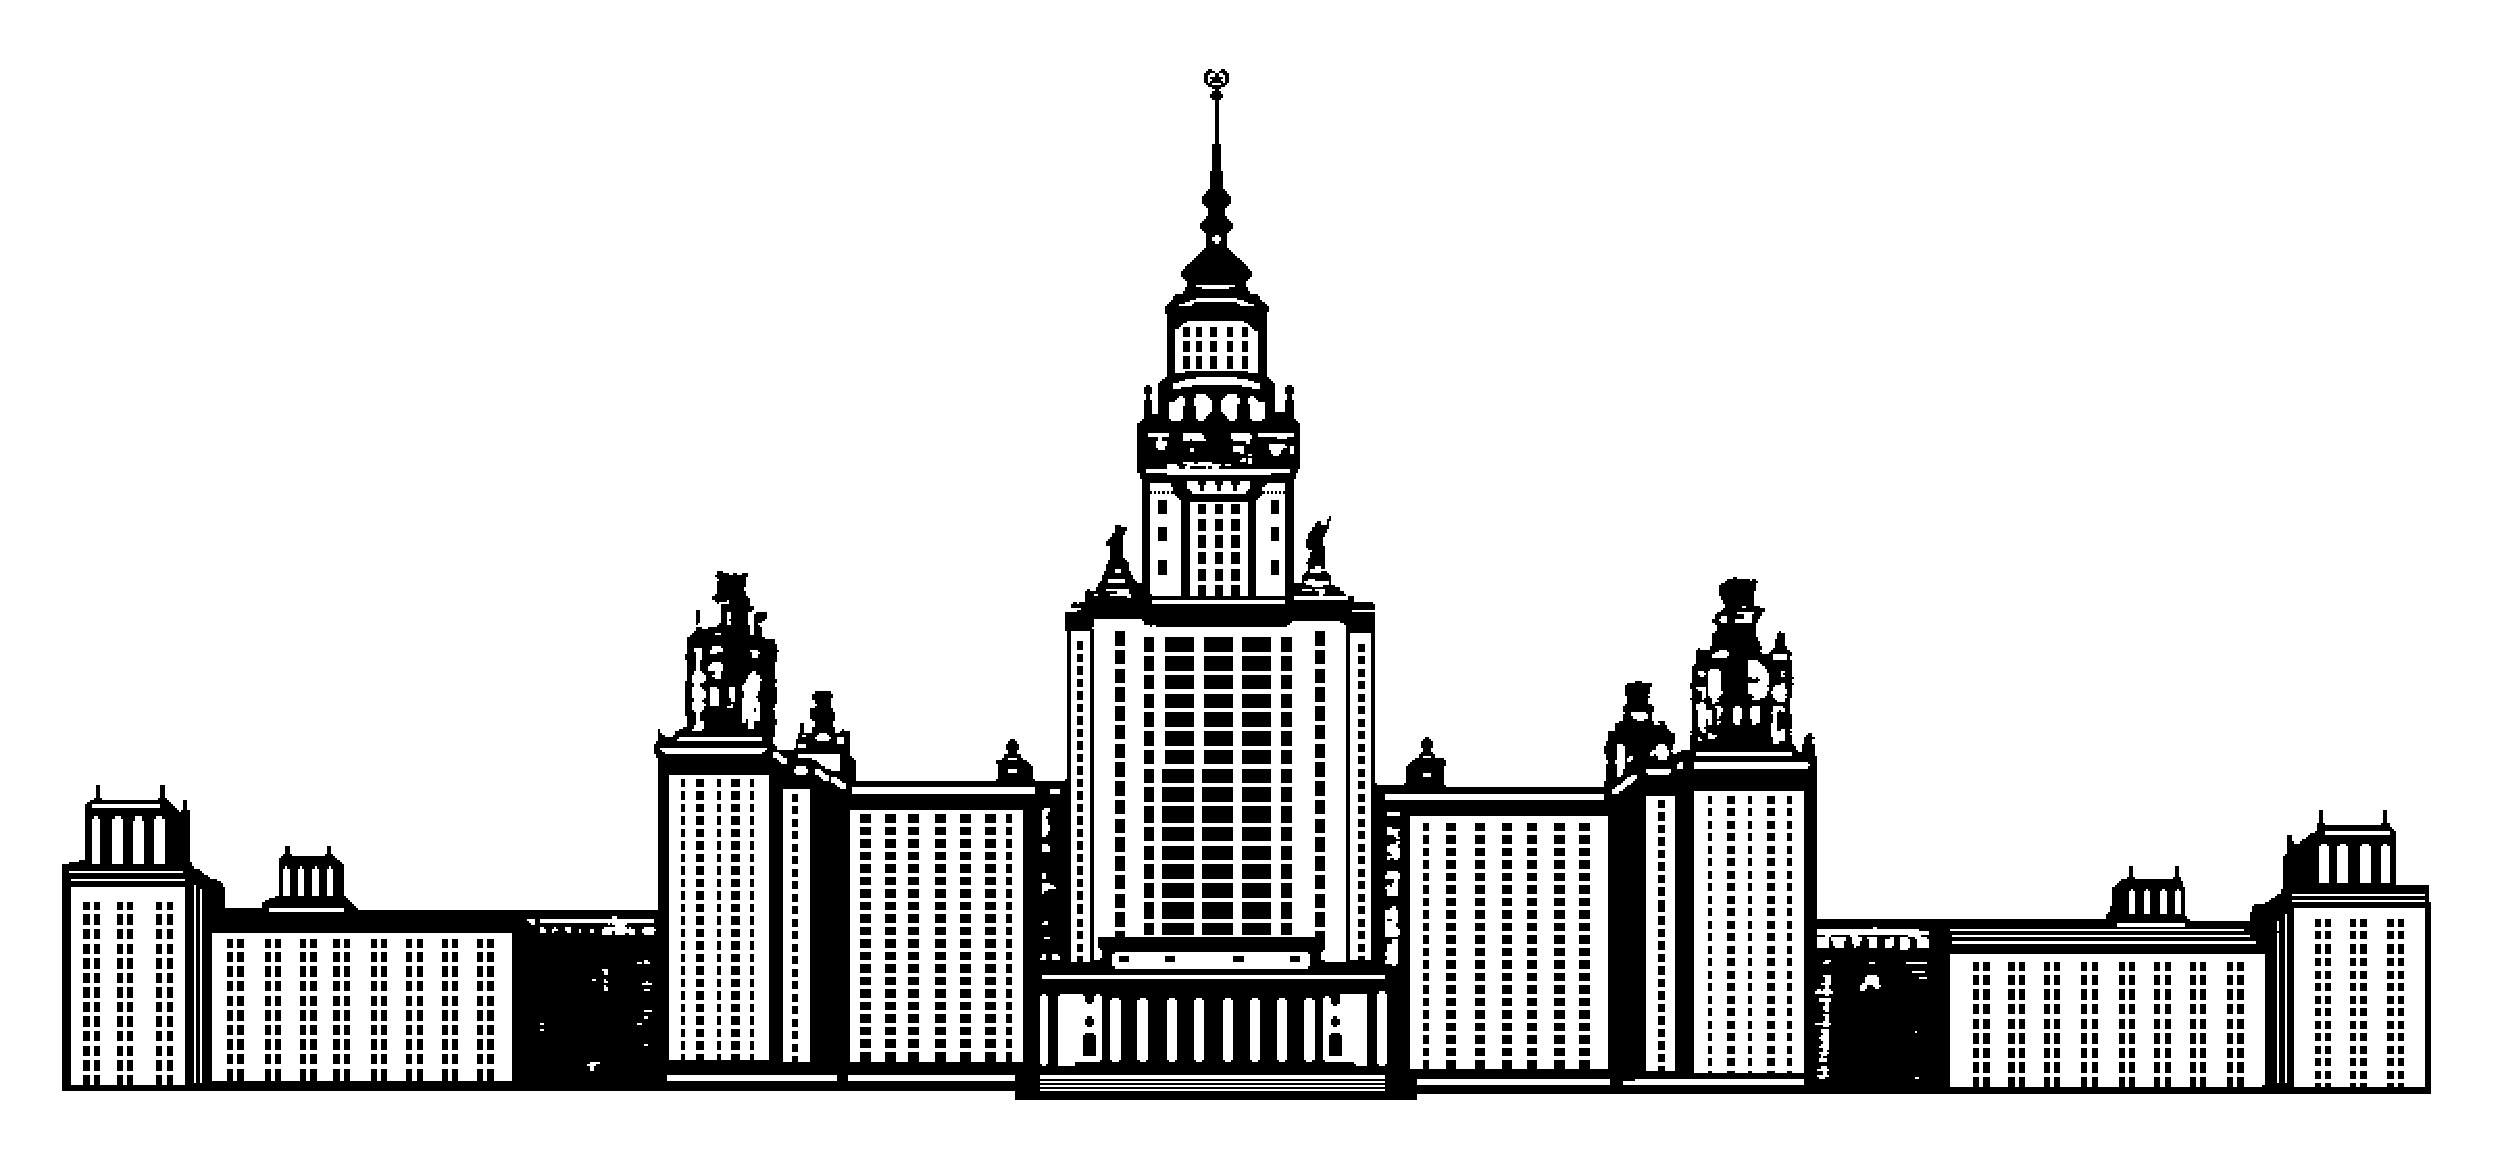
\includegraphics[width=75mm]{msu.eps}\\
    \bigskip
    Московский государственный университет им. Ломоносова\\
    Факультет вычислительной математики и кибернетики\\
    Кафедра Математических Методов Прогнозирования\\[10mm]
    
    Федоров Илья Сергеевич \\
    \textsf{\large\bfseries
        Построение поисковой системы для интернет магазина
    }\\[10mm]
    
    ВЫПУСКНАЯ КВАЛИФИКАЦИОННАЯ РАБОТА
    \vspace{\fill}
    \begin{flushright}
        \parbox{0.5\textwidth}{
            \textbf{Научный руководитель:}\\
            д.ф-м.н., профессор\\
            \emph{А. Г. Дьяконов}
        }
    \end{flushright}

    \vspace{\fill}
    Москва, 2021
\end{center}
\end{titlepage}

\newpage
\renewcommand{\contentsname}{Содержание}
\addtocounter{page}{1}
\tableofcontents

\newpage
\section{Введение}

Современный технологический прогресс неразрывно связан с быстрым доступом к информации. Ежедневно поисковые системы обрабатывают миллиарды запросов от колоссального количества людей по всему миру, а их базы данных исчисляются десятками миллионов терабайт. И хотя поисковые системы, безусловно, стоит считать одним из главных достижений человечества за последние десятилетия, задача получения данных по запросу возникает и в других приложениях меньших масштабов, к примеру, задача выдачи подходящих под запрос пользователя товаров в интернет-магазине. 

Основной целью данной работы является исследование подходов к построению поисковой системы для абстрактного интернет-магазина с использованием современных технологий глубокого обучения и нейронных сетей. Безусловно, для её решения, существуют (и активно применяются на практике) методы, никак не использующие машинное обучение. Однако рост интереса исследователей и бизнеса к глубокому обучению, а также активное развитие вычислительной техники, позволяющие обучать глубокие нейросети, способствуют развитию применения технологий интеллектуальной обработки естественного языка в данной области. В качестве преимуществ подходов, использующих нейросетевые технологии для обработки пользовательских запросов, можно отметить зачастую более стабильную работу системы с точки зрения устойчивости к зашумленным входным данным (к примеру, в случае, когда клиент допустил опечатку в запросе).

В исследовании рассмотрены некоторые из существующих подходов к приложению технологий глубокого обучения к задаче построения поисковой системы для интернет-магазина, описаны особенности и сложности сбора данных в контесте решаемой задачи, предложена архитектура поисковой системы, основанная на BERT\cite{bert}, а также представлены результаты экспериментов и значения метрик для предложенной модели. 

\section{Постановка задачи}

Существует множество подходов к построению поисковой системы для интернет-магазина. Во многом они зависят от способа представления товаров в базе данных. К примеру, они могут описываться большим количеством признаков (такими как название, бренд, страна-производитель, размеры, цвет и т.д.), а могут лишь одной текстовой строкой - описанием, в котором, как предполагается, содержится вся информация о товаре.

Основным случаем, рассмотренным в данной работе, является модель данных, в которой товары в базе магазина описываются тремя признаками: описание товара, название товара и название бренда. Примеры представлены в таблице 1.

\begin{table}[H]
\begin{center}
    \scalebox{0.7}{
    \begin{tabular}{||c c c c||} 
    \hline
    № & Описание товара & Название товара & Бренд \\ [0.5ex] 
    \hline\hline
    1 & Смартфон Apple iPhone 5S 16Gb Space Gray (ME432RU/A) & Смартфон & Apple \\ 
    \hline
    2 & Варенье Вкусвилл брусника - апельсин, 310 г & Варенье & Вкусвилл \\
    \hline
    3 & Женские кроссовки CALVIN KLEIN JEANS & Кроссовки & CALVIN KLEIN JEANS \\
    \hline
    4 & Гриль Bosch TFB3323V & Гриль & Bosch \\
    \hline
    5 & TELEFUNKEN / Портативная колонка TF-1234B & Портативная колонка & TELEFUNKEN \\ [1ex] 
    \hline
    
    \end{tabular}}
    \caption{Пример данных в базе интернет-магазина}
\end{center}
\end{table}

\noindent 
Данная модель является некоторым промежуточным вариантом между тем случаем, когда товар описывается большим количеством различных признаков, и тем, когда товар описывается лишь одной текстовой строкой (то, что в рассматриваемой модели называется описанием товара). Мотивация выбора такой модели будет описана в подразделе «Особенности сбора данных».\textbf{}

Будем считать, что интернет-магазин имеет доступ к базе данных с описанной выше моделью, а также некоторый сайт, который позволяет получать текстовые запросы от клиентов (пользователей). Пользователь задает свой запрос в текстовом виде на естественном языке. В ответ поисковая система должна предоставить некоторый список товаров из базы, которые являются наиболее релевантными запросу пользователя. Мы предполагаем, что пользователь вводит запрос, содержащий в себе слова, характеризующие товар. Безусловно, идеальным запросом являлось бы точное описание товара из базы данных магазина, тогда мы бы смогли произвести явный поиск по существующим наименованиям и выдать точный результат. Однако на практике пользователь никогда не будет знать, как именно нужный ему товар представлен в базе, а также довольно часто клиента интересует не конкретный товар, а некоторый каталог релевантных его запросу товаров. К примеру, его может интересовать чайник (без уточнения бренда) или все продукты компании Apple (без уточнения названия товара). Таким образом, будем предполагать, что запрос пользователя будет состоять из трех компонент, каждая из которых может как присутствовать, так и отсутствовать: название товара, название бренда и уточняющая информация. Примеры запросов с соответствующим разделением слов по указанным трем компонентам представлены в таблице 2.

\begin{table}[H]
\begin{center}
    \scalebox{0.8}{
    \begin{tabular}{||c c c c c||} 
    \hline
    № & Запрос & Название товара & Бренд & Уточняющая информация \\ [0.5ex] 
    \hline\hline
    1 & чехол для iphone 6 & чехол & (нет) & для iphone 6  \\ 
    \hline
    2 & смартфоны xiaomi & смартфоны & xiaomi & (нет)  \\ 
    \hline
    3 & чайник электрический маленький & чайник & (нет) & электрический маленький  \\ 
    \hline
    4 & apple iphone 7 & (нет) & apple & iphone 7  \\ 
    \hline
    5 & футболки мужские с принтом & футболки & (нет) & мужские с принтом  \\ 
    \hline
    
    \end{tabular}}
    \caption{Примеры запросов и соответствующих им смысловых частей}
\end{center}
\end{table}

Исходя из описанной выше модели данных в базе магазина и предполагаемой стуктуры запроса пользователя, поставим задачу построения поисковой системы следующим образом. В запросе пользователя необходимо выделялить следующие сущности: название товара, название бренда и уточняющую информацию. После выделения этих компонент, соответствующим образом ведется поиск по базе товаров магазина. К примеру, если выделен и бренд B, и название товара I, то пользователю выдается некоторая выборка товаров, имеющих бренд B и название товара I (это легко сделать, поскольку мы предположили, что данные признаки уже выделены в базе данных интернет-магазина). Если же выделено, к примеру, только название товара I, то стоит показать пользователю выборку товаров с названием I, вне зависимости от бренда. Данная задача давно известна в области обработки естественного языка (natural language processing, NLP) как распознавание именованных сущностей (named entity recognition, NER).

Отдельного внимания заслуживает «уточняющая информация». Поскольку данная компонента может изменяться в слишком широких масштабах (так как для разных категорий товаров подробности описания могут сильно отличаться, к примеру, для чайников важен объем, а для планшетов -- размер экрана), попытки привести её в унифицированный вид могут быть достаточно затруднительными (подробнее об этом будет сказано в следующем подразделе). В связи с этим данная информация должна учитываться в поисковой выдаче, которая была отфильтрована названием товара и бренда, некоторым особым образом.

Описанный выше алгоритм можно записать по шагам:

\begin{enumerate}
    \item Пользователь задает текстовый запрос.
    \item С помощью нейросети из запроса выделяется название товара и название бренда.
    \item По базе товаров магазина выполняется поиск: определяется множество товаров, которые имеют выделенное на прошлом шаге название и бренд.
    \item С помощью дополнительных алгоритмов полученное множество товаров сортируется с учетом «уточняющей информации».
    \item Пользователю выдается отсортированный список товаров.
\end{enumerate}

\noindent В ходе проведения исследования автор столкнулся с рядом трудностей, которые осложняют построение системы, которая бы выполняла сразу все вышеперечисленные пункты. Подробнее указанные затруднения будут описаны в последующих разделах. В связи с этим, целью данной работы является второй пункт из списка выше: построение нейросети, выполняющей задачу распознавания именованных сущностей в запросе пользователя. В сущности, такая модель становится «ядром» описываемой системы, а остальные пункты легко реализуются при наличии соответствующих ресурсов и наборов данных.

\section{Обзор существующих работ}
Приведем краткий обзор некоторых работ, связанных с данным исследованием.
\subsection{Подход на основе рекуррентных нейросетей}
Наиболее близкой по задаче и методу решения является статья \cite{ner}, выпущенная командой сотрудников компании The Home Depot (https://www.homedepot.com/), которая занимается продажей товаров для дома, ремонта и строительства. Авторы рассматривают в точности такую же постановку задачи, как и в данной работе (классификация слов в запросе пользователя на название товаров, бренд и прочие слова). В рамках статьи они представили цельное (end-to-end) решение. Было предложено, как оптимальным образом организовать создание обучающих датасетов, была обучена нейросеть для распознавания именованных сущностей, а также представлены некоторые показатели метрик качества. Рассмотрим подробнее каждый из этих этапов. 

\textbf{Подготовка данных.} С учетом того факта, что в качестве модели классификации будет использоваться глубокая нейросеть, авторы статьи выдвигают три требования к обучающему датасету.

\begin{enumerate}
    \item Большое количество данных
    \item Высокое качество разметки
    \item Широкое покрытие меток классов (названий товаров и брендов)
\end{enumerate}

\noindent Идеальным решением для такого перечня требований стал бы большой набор данных, размеченных вручную. Однако разметка текстовых данных (особенно с учетом того факта, что иногда потребуется дополнительно проводить поиск: является ли некоторое слово брендом или неизвестным разметчику товаров) является достаточно сложной и дорогостоящей процедурой. В связи с этим, авторы предлагают составить обучающий датасет из трех компонент:

\begin{enumerate}
    \item Размеченные автоматическими эвристическими методами данные.
    \item Размеченные вручную запросы.
    \item Запросы, состоящие только из бренда или названия товара.
\end{enumerate}

\noindent В первой компоненте для автоматической разметки используются детерминированные алгоритмы, основанные на сопоставлении в запросах пользователей слов с названиями брендов и товаров. Вторая часть, как и следует из названия, состоит из размеченных человеком данных, однако, как уже было отмечено, этот процесс трудозатратен, поэтому данная компонента сравнительно невелика в размерах. Третья часть призвана отвечать третьему требованию, а именно пополнять «кругозор» модели редко встречающимися товарами и брендами. Подробнее о том, как именно будут использоваться три указанных поднабора данных, будет сказано ниже.

\textbf{Модель.} В ходе экспериментов авторы тестировали различные нейросетевые архитектуры, в основе которых лежат рекуррентные нейросети (recurrent neural networks, RNN). Ещё с конца прошлого века было известно, что классические RNN обладают рядом недостатков: при их обучении стохастические градиенты часто, проходя через слои сети, начинают быстро затухать (в связи с чем модель «забывает» контекст очередного входа довольно быстро), а иногда, наоборот, «взрываются», когда модуль градиента экспоненциально увеличивается на каждом шаге алгоритма обратного распространения. В связи с обозначенными проблемами, на практике чаще всего применяются модификации RNN: LSTM (Long-Short Term Memory) \cite{lstm}  и GRU (Gated Recurrent Unit) \cite{gru}. В задачах, в которых заранее целиком известна входная последовательность (например, NER, но не предсказание временных рядов), рекуррентные модели также часто модифицируют до их двунаправленных версией: BiLSTM (Bidirectional LSTM) и BiGRU (Bidirectional GRU). Основным отличием является наличие в архитектуре двух нейросетей, в одну из которых входная последовательность поступает в прямом порядке, а в другую --- в обратном. Это способствует улавливанию моделью двухстороннего контекста очередного элемента входа. 

\begin{figure}[H]
\begin{center}
  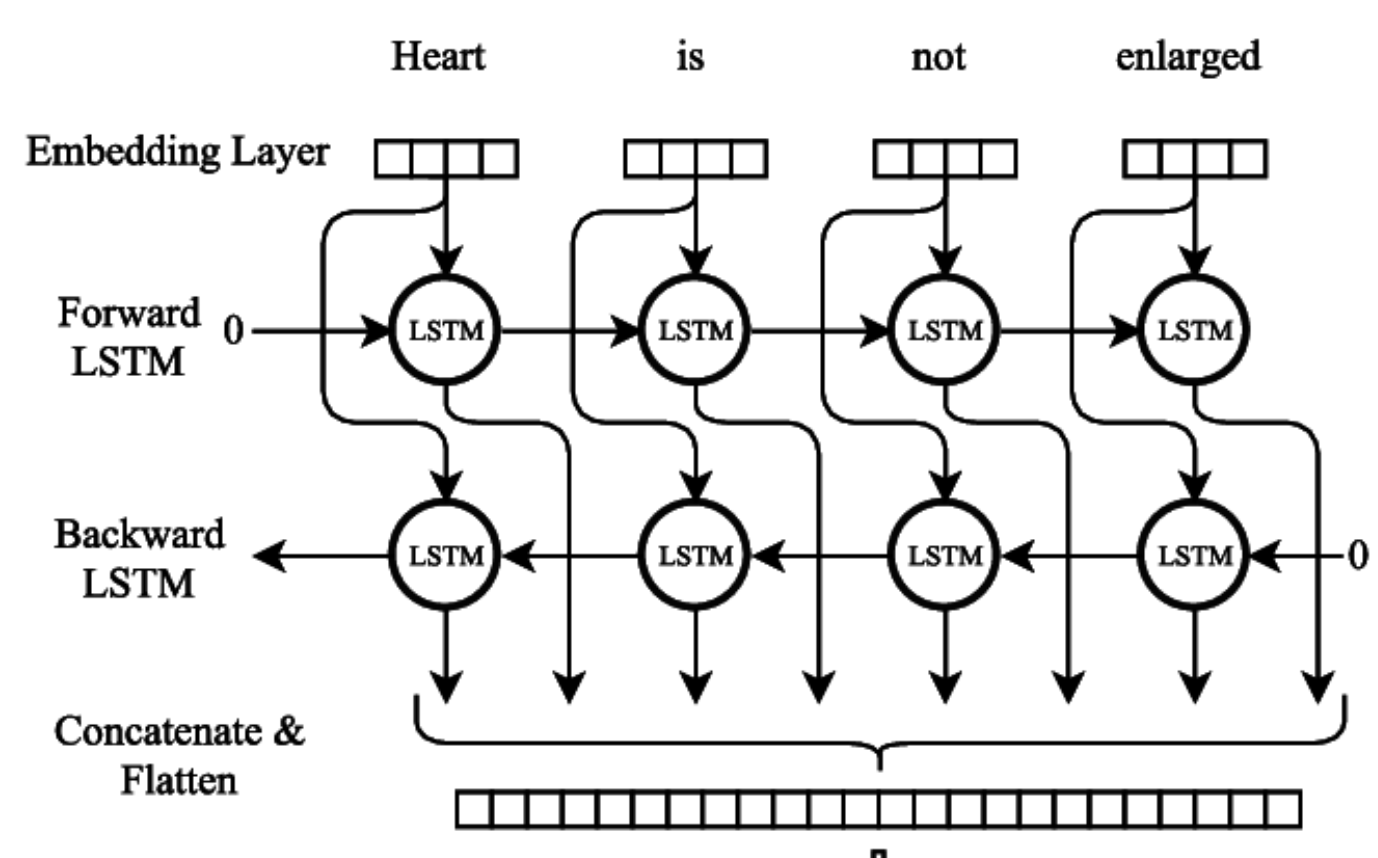
\includegraphics[width=0.4\textwidth]{bilstm.png}
  \caption{BiLSTM}
\end{center}
\end{figure}

Для построения финальной модели, авторы рассматриваемой статьи комбинируют указанные выше двунаправленные архитектуры. А именно, для составления векторных представлений слов (эмбеддингов) в предложении используется посимвольная BiLSTM (рис. 2), а для решения задачи распознавания именованных сущностей BiGRU с CRF\cite{crf} (Conditional Random Field) слоем (рис. 3), на вход которой подается последовательность токенов, полученных из слов после прогонки через первую нейросеть.

\begin{figure}[H]
\begin{center}
  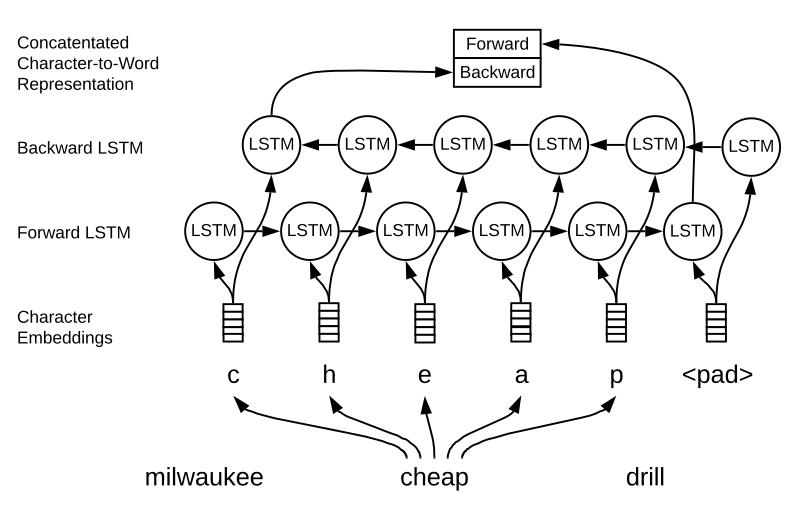
\includegraphics[width=0.65\textwidth]{pap_emb.jpg}
  \caption{Посимвольная BiLSTM нейросеть для получения эмбеддингов}
\end{center}
\end{figure}

\begin{figure}[H]
\begin{center}
  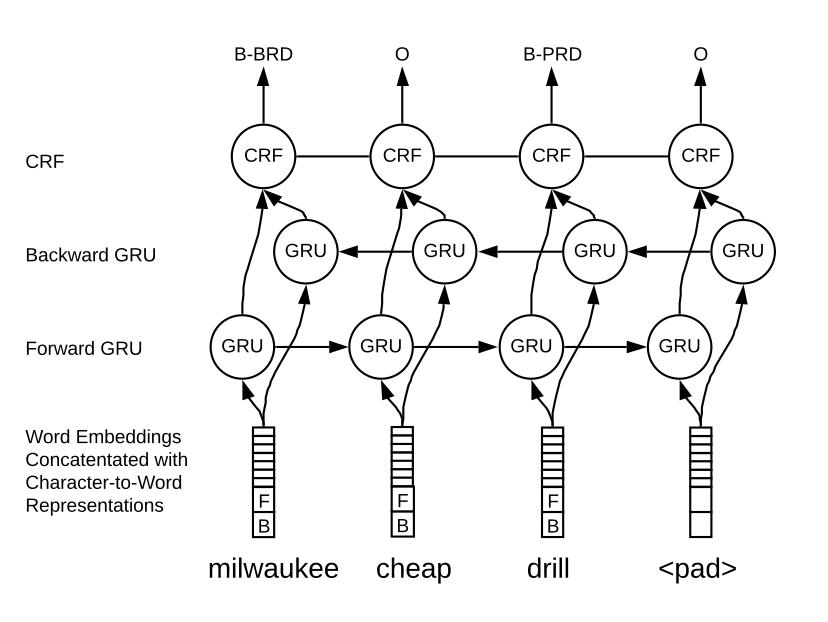
\includegraphics[width=0.65\textwidth]{pap_net.jpg}
  \caption{BiGRU-CRF для NER}
\end{center}
\end{figure}

\textbf{Итеративный процесс обучения.} После того как были описаны входные датасеты и модель, мы можем рассмотреть предлагаемый авторами статьи процесс обучения итоговой системы. Все её компоненты представлены на рисунке 4.

\begin{figure}[H]
\begin{center}
  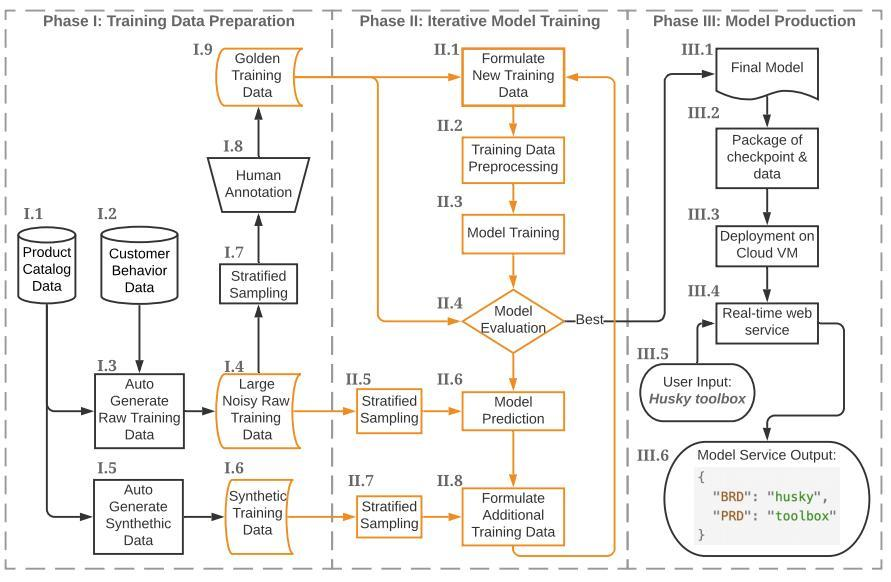
\includegraphics[width=0.9\textwidth]{loop.jpg}
  \caption{Левый столбец --- датасеты. Центральный --- цикл обучения. Правый --- особенности развертки модели в бизнес.}
\end{center}
\end{figure}

\noindent Первая итерация начинается с вручную размеченного датасета («золотого» датасета, так как данные размечать дорого) (I.9). 15\% от этих данных случайным образом откладываются в качестве тестовой выборки; остальные данные случайным образом разделяются на обучающие (90\% оставшихся данных) и валидационные («dev») данные (10\%). Затем данные для обучения предобрабатываются (II.2). На следующем этапе (II.3) модель обучается до тех пор, пока F1-мера качества не перестанет улучшаться на валидационной выборке, либо пока не будет достигнуто максимальное число итераций (эпох). Далее выполняется оценка качества на тестовой выборке (II.4). Если выполнен некоторый критерий остановки (достигнуто максимальное число итераций, или модель достигла необходимого качества), то процесс завершается. Иначе алгоритм переходит на шаги расширения обучающего датасета (II.6 и II.7). На этапе II.6 из составленной с помощью эвристических алгоритмов компоненты (I.4) данных случайным образом сэплируется некоторая подвыборка. Текущая модель делает предсказание меток классов. Если метки, полученный эвристическим алгоритмом, а также метки модели совпадают, то такой сэмпл добавляется в обучающий датасет. На этапе II.7 к нему случайным образом дополнительно добавляются сэмплы, состоящие только из бренда или названия товара. 

\textbf{Результаты.} На рис. 5 изображена таблица, представленная авторами в статье. Как было отмечено выше, лучшие результаты показала архитектура, использующая 2 нейросети: посимвольная BiLSTM для построения векторных представлений слов и BiGRU-CRF для непосредственного распознавания именованных сущностей. В качестве метрики используется F1-мера (среднее гармоническое между точностью и полнотой классификации слов в запросе, усредненное по всем запросам в соответствующем наборе данных).

\begin{figure}[H]
\begin{center}
  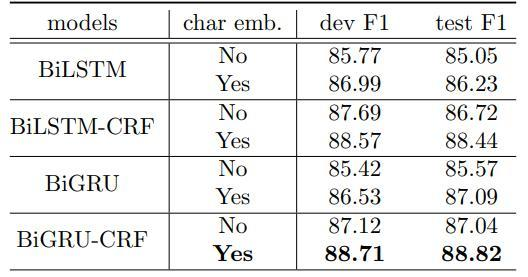
\includegraphics[width=0.5\textwidth]{tab.jpg}
  \caption{Результаты авторов статьи}
\end{center}
\end{figure}

\subsection{BERT}

Ключевым отличием данной работы от исследования, описанного в предыдущем разделе, является использование более современной нейросетевой архитектуры, которая называется BERT (Bidirectional Encoder Representations from Transformers). Архитектура была предложена\cite{bert} в 2018 году и стала активно применяться во многих задачах обработки естественного языка, для решения которых используются нейросети. Поскольку эта модель лежит в основе предлагаемого в данной работе решения, кратко опишем её ключевые принципы работы.\\

\textbf{Архитектура Transformer.} Революционной для области глубокого обучения в обработке естественного языка стала статья \cite{transformer}, вышедшая в 2017 году. В статье была описана архитектура Transformer --- первая успешная модель для задачи машинного перевода, не использующая рекуррентные нейросети. Рассмотрим более подробно данную архитектуру, поскольку  она тесно связана с нужным нам BERT'ом.

\begin{figure}[H]
\begin{center}
  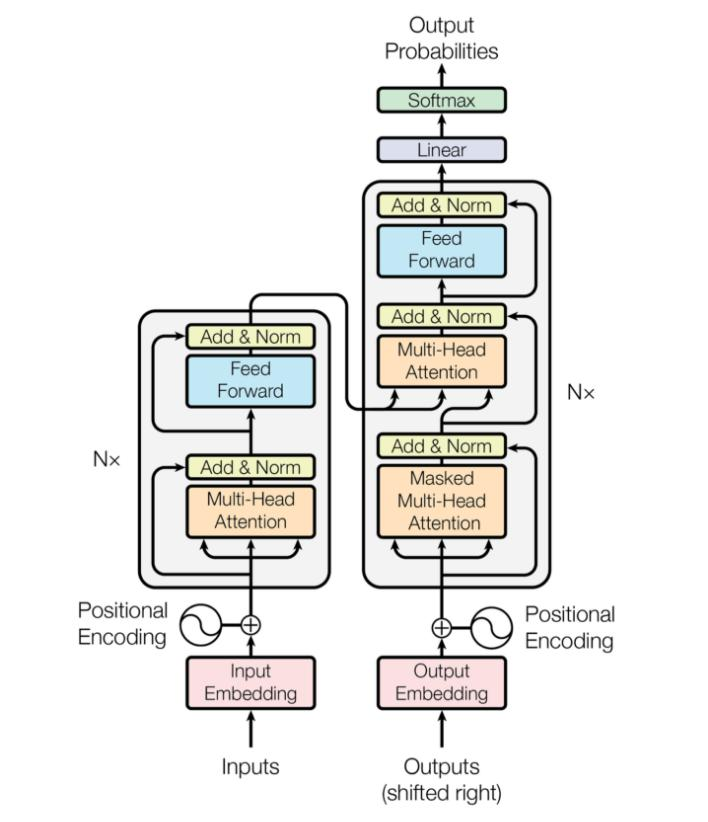
\includegraphics[width=0.5\textwidth]{transformer.jpg}
  \caption{Архитектура Transformer}
\end{center}
\end{figure}

\noindent На рисунке 6 изображена схема трансформера: левый блок представляет собой один слой энкодера, а правый --- один слой декодера. Для понимания BERT нас будет интересовать только энкодер. Опишем, из чего он состоит.

Механизм внимания (Attention). Идея Attention довольно проста: имея наборы векторов-ключей и соответствующих им векторов-значений ($K$, $V$), а также вектор-запрос $q$, требуется найти в $K$ вектор, наиболее похожий на $q$, и выдать соответствующий ему вектор-значение из $V$. На практике в качестве меры схожести используется скалярное произведение. Поскольку данный механизм хочется использовать в нейронных сетях, операцию взятия ключа по значению заменяют на суммирование всех значений с некоторыми весами, чтобы данная операция была дифференцируема. В свою очередь указанные веса получаются применением функции softmax к скалярным произведениям векторов из $K$ и $q$. Описанный механизм легко записать в матричном виде:$$Attention(q, K, V) = \softmax \left(qK^T \right) V,$$
где в $K$ и $V$ векторы записаны по строкам, а $q$ --- это запроса-строка. На практике обычно в «головку» внимания приходит не один вектор-запрос, а несколько, поэтому их удобно также собрать в единую матрицу $Q$. Также дополнительно будем нормировать аргумент softmax на некоторую константу $\beta$ (на практике $\beta = \sqrt{d}$, где $d$ - размерность ключей), для стабильности вычислений. В итоге получим формулу:
$$Attention(Q, K, V) = \softmax \left(\frac{QK^T}{\beta} \right) V.$$
В трансформере используется модификация данного механизма: многоголовое внимание (MultiHead Attention). Основным отличием «многоголового» внимания является наличие нескольких параллельно работающих головок Attention.

\begin{figure}[H]
	\begin{center}
		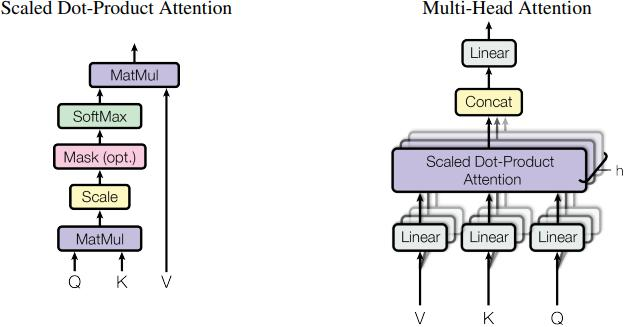
\includegraphics[scale=0.65]{mh2.jpg}
	\end{center}
	\caption{Схема механизма внимания (слева) и многоголового внимания (справа) \cite{transformer}}
\end{figure}

\noindent Для того, чтобы получать разные результаты, исходные матрицы $Q$, $K$ и $V$ линейным образом преобразуются. После этого для каждой тройки таких матриц применяется обычная головка Attention. Далее полученные результаты конкатенируются, и снова преобразуются линейным образом. Все перечисленные этапы можно описать несколькими простыми формулами:
$$\mathrm{MultiHead} (Q, K, V) = \mathrm{Concat}(\mathrm{head}_1, \dots, \mathrm{head}_h) W^O$$
$$\mathrm{where} \enspace \mathrm{head}_i = \mathrm{Attention}(QW_i^Q, KW_i^K, VW_i^V)$$
\noindent Где матрицы $W^O$, $W_i^Q$, $W_i^K$, $W_i^V$ --- обучаемые параметры.

Энкодер. Энкодер состоит из нескольких (в оригинальной статье $N = 6$) идентичных слоев. Каждый из них имеет архитектуру, изображенную слева на рисунке 6. В свою очередь каждый слой имеет два подслоя. Первым из них является Multi-Head Attention, а вторым --- обычная полносвязная нейросеть. Выход каждого слоя складывается со своим входом, а к полученной сумме применяется нормализация по слою (Layer Normalization). Данный механизм (который называется skip-connections) нужен для решения проблемы затухающих градиентов. 


\textbf{Архитектура BERT.} В сущности, BERT\cite{bert} представляет собой энкодер от трансформера. Входная последовательность проходит через слои, каждый слой выполняет над эмбеддингами некоторое преобразование. На выходе сети получаются транформированные эмбеддинги для входной последовательности токенов.

\begin{figure}[H]
	\begin{center}
		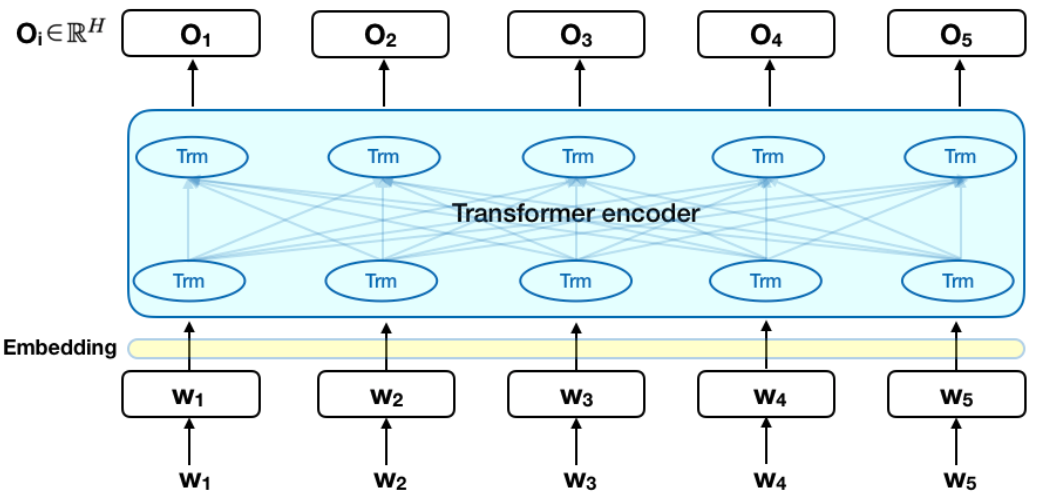
\includegraphics[scale=0.3]{trans2.png}
	\end{center}
	\caption{Преобразование токенов через BERT, изображение с сайта lyrn.ai, статья от Rani Horev}
\end{figure}

Ключевой особенностью данной модели является возможность её использования для многочисленных задач NLP. Этап обучения разбивается на 2 этапа:
\begin{enumerate}
    \item Предобучение (pre-train). На данном этапе модель обучается на большом корпусе неразмеченных текстов.
    \item Дообучение (fine-tuning). Предобученный на предыдущем этапе BERT дообучается на конкретную задачу (к примеру, классификация текстов или NER).
\end{enumerate}

\noindent Данная парадигма называется «передача модели обучения» (на практике обычно используется название на английском --- transfer learning). Как показывают многочисленные эксперименты, модель, предварительно обученная на некоторые задачи на большом неразмеченном наборе текстов, а потом дообученная на конкретную (downstream) задачу, показывает гораздо лучшие результаты, чем модель, обученная только на некоторую специфичную задачу без предобучения. Рассмотрим более подробно данные этапы для BERT.

\textbf{Предобучение (pre-train).} Предобучение BERT на большом корпусе неразмеченных данных выполняется с помощью решения двух задач:
\begin{enumerate}
    \item Предсказание замаскированных слов (Masked Language Modelling, MLM)
    \item Классификация: являются ли два предложения идущими друг за другом в тексте (Next Sentence Prediction, NSP).
\end{enumerate}

\noindent Предсказание замаскированных слов. Классическая проблема в однонаправленных языковых моделях (к примеру, в рекуррентных нейросетях): модель видит контекст слова только с одной стороны. Если же использовать двунаправленный подход, то возникает проблема переобучения, поскольку информация о предсказываемом слове содержится в одном из контекстов (левом или правом). Авторы BERT предлагают следующий подход: некоторая доля слов в предложениях закрываются масками, а модель должна их предсказать:

\begin{figure}[H]
	\begin{center}
		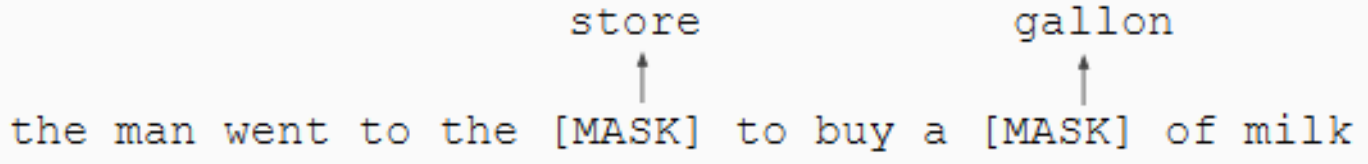
\includegraphics[scale=0.4]{masked.png}
	\end{center}
	\caption{Задача определения замаскированных слов}
\end{figure}


\noindent Классификация: является ли предложение А продолжением предложения Б. Смысл следует из названия.  
\begin{figure}[H]
	\begin{center}
		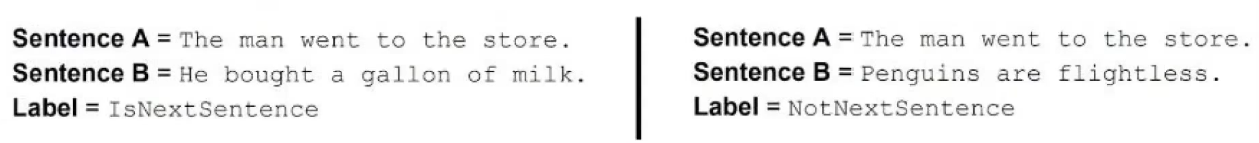
\includegraphics[scale=0.5]{nsp.png}
	\end{center}
	\caption{Задача NSP (Next Sentence Prediction)}
\end{figure}

\noindent Обученный для решения этих задач BERT оказывается достаточно интеллектуальной системой: задача восстановления замаскированных слов позволяет ей «понимать» связи между словами в предложении, а задача NSP позволяет ей устанавливать связи между целыми предложениями. Важно отметить, что данные, на которых выполняется pre-train BERT не требуют разметки, что позволяет обучать его на огромном количестве данных. В связи с этим BERT активно применяется для решения множества задач.\\

\noindent \textit{Замечание.} Как показали эксперименты в оригинальной статье, задача NSP не несет существенного вклада в качество модели, поэтому часто на практике на этапе предобучения её пропускают.\\

\textbf{Дообучение (fine-tuning).} После того как модель предобучена на большом корпусе текстов, архитектура BERT незначительно изменяется для решения необходимых задач. В частности, для распознавания именованных сущностей (то есть, по сути, классификации токенов), достаточно добавить полносвязный линейный слой и слой softmax, которые принимают на вход прошедшие через BERT входные токены. Помимо NER, BERT часто используется для следующих задач:
\begin{itemize}
    \item Классификация входных последовательностей,
    \item Ответы на вопросы (QA),
    \item Natural language inference (NLI) --- классификация: следует ли из предложения-посылки предложение-вывод
\end{itemize}
\noindent и т.д.

\section{Данные}
\subsection{Особенности сбора данных}

Проведение некоммерческих исследований в рассматриваемой в данной работе области затрудняется в связи с высокой коммерциализацией. Необходимые для построения поисковых систем данные могут быть получены единственным образом: путем выгрузки данных из баз реальных интернет-магазинов. Чаще всего компании не стремятся делиться подобной информацией, поскольку она может быть использована конкурентами. Из постановки задачи следует, что для построения поисковой системы необходимы как минимум два набора данных: база товаров, а также примеры запросов пользователей. Опишем затруднения, которые возникли во время сбора указанных датасетов.

\textbf{База товаров.} На первый взгляд может показаться, что собрать такие данные довольно просто, ведь все интернет-магазины имеют каталоги товаров, а для каждого товара указаны как минимум название, описание, категория и чаще всего бренд. Однако на практике подавляющее большинство компаний стараются защитать свои сайты от автоматического сбора данных (скрапинга, парсинга). Безусловно, такие защиты можно обойти, но при этом они достаточно сильно затрудняют процесс получения необходимых датасетов. Кроме того, разные категории товаров описываются значительно отличающимися друг от друга наборами признаков. К примеру, для одежды важны такие параметры как размер, цвет, материал, бренд и страна-производитель, а для смартфона -- мощность процессора, объем памяти, размеры экрана, бренд, модель и т.д. Таким образом, при попытке сбора максимально детализированной информации о товарах (то есть когда товар описывается большим количеством признаков), гипотетический исследователь может столкнуться с тем, что в собранных им данных количество признаков невероятно велико, и для получения хоть сколько-то репрезентативной выборки необходимо спарсить практически все товары с сайта магазина, что в условиях некоммерческой разработки просто невозможно (из-за описанных выше проблем с защитой сайтов). Именно этот факт мотивирует предложенную модель данных для базы товаров, предложенную в разделе с постановкой задачи. Однако, если построение поисковой системы ведет уже существующий интернет-магазин с большим количеством детализированных примеров, модель с более подробным описанием каждого товара была бы возможна (и, скорей всего, более успешна).

\textbf{Запросы пользователей.} Если сведения о товарах, хоть и с трудом, но можно получить из открытых источников, то текстовые запросы клиентов в поиковую строку интернет-магазина являются полностью закрытой для сторонних лиц информацией. Автор данной работы провел в поисках открытых данных подобного рода более двух недель, и ничего похожего найдено не было. Однако был найден способ добывать текстовые запросы, наиболее похожие на необходимые. Довольно часто пользователи ищут товары не непосредственно на сайтах интернет-магазинах, а вводят свой запрос в поисковые системы вроде Google или Яндекса. При этом, если взять запросы, по которым совершаются переходы на крупные интернет-магазины (или их агрегаторы), какие как Ozon, Яндекс.Маркет и т.д., то окажется, что почти все такие запросы представляют собой как раз те самые текстовые строки, которые нам нужны (быть может, с некоторыми дополнительными словами, к примеру "купить"). Однако существуют сервисы (к примеру, ahrefs.com), которые позволяют анализировать и предсказывать переходы на сайты с поисковых систем. При этом подобные сервисы часто продают подобные данные. Именно таким образом можно собрать некоторую базу поисковых запросов в интернет-магазинах, не обращаясь к компаниям напрямую.

\subsection{Описание собранных наборов данных}

\textbf{База названий товаров.} Часть данных была получена путем сбора названий, категорий и брендов с сайтов крупных интернет-магазинов Ozon, BERU, Яндекс.Маркет, Юлмарт. С указанных площадок было собрано порядка 450.000 наименований. Отметим, что для построения основной компоненты поисковой системы (а именно глубокой нейронной сети для задачи NER) будут использоваться лишь текстовые строки, содержащие всю информацию о товаре (то, что выше было названо описанием товара). Значительная часть товаров принадлежит разделу «Электроника». Пример данных из данной части выборки -- в таблице 3.

\begin{table}[H]
\begin{center}
    \scalebox{0.9}{
    \begin{tabular}{||c c||} 
    \hline
    № & Описание товара \\ [0.5ex] 
    \hline\hline
    1 & Смартфон Sony Xperia Z2 D6503 Purple \\ 
    \hline
    2 & Чайник Bosch TWK7808, золотистый   \\ 
    \hline
    3 & a4tech / Мышь Bloody P80 Pro  \\ 
    \hline
    4 & Игровая консоль PlayStation 5, белый  \\ 
    \hline
    
    \end{tabular}}
    \caption{Примеры товаров с сайтов Ozon, BERU, Яндекс.Маркет, Юлмарт}
\end{center}
\end{table}


\noindent Помимо собранных данных из открытых источников, были использованы данные, предоставленные на соревновании DataFusion, проходившем на площадке boosters.pro с 27 января 2021 года по 27 марта 2021 года. В задаче требовалось определить бренд товара по его текстовому описанию в чеке. Всего в датасете были представлены 3.1 млн подобных текстовых строк. Основная часть наименований является названиями продуктов питания, однако встречаются товары и из других разделов. Некоторые примеры из этого набора данных представлены в таблице 4.

\begin{table}[H]
\begin{center}
    \scalebox{0.9}{
    \begin{tabular}{||c c||} 
    \hline
    № & Описание товара \\ [0.5ex] 
    \hline\hline
    1 & 20 БРЮКИ МУЖ / J Lin / 72 MC 1 \\ 
    \hline
    2 & " Русский Аппетит " Суп борщ 50 гр .   \\ 
    \hline
    3 & Йогурт Даниссимо фантазия 105 г хрустящие шарики  \\ 
    \hline
    4 & Штора рулонная " Декор белый 57 * 160 см  \\ 
    \hline
    
    \end{tabular}}
    \caption{Примеры товаров из даннных с соревнования DataFusion}
\end{center}
\end{table}

\textbf{Запросы пользователей.} Изначально, запросы собирались с помощью метода описанного в предыдущем подразделе. Таким образом было собрано порядка 50.000 запросов среднего качества. Однако, к счастью, автору работы удалось связаться с компанией KazanExpress (https://kazanexpress.ru), которая на безвозмедной основе передала для проведения некоммерческих исследований датасет запросов пользователей размером 3.7 млн записей. Примеры запросов -- в таблице 5.

\begin{table}[H]
\begin{center}
    \scalebox{0.9}{
    \begin{tabular}{||c c||} 
    \hline
    № & Запрос \\ [0.5ex] 
    \hline\hline
    1 & ботинки рабочие \\ 
    \hline
    2 & чехол для iphone  \\ 
    \hline
    3 & redmi note 9  \\ 
    \hline
    4 & сменная головка для бритвы philips  \\ 
    \hline
    5 & капсулы для кофемашин bosch tassimo  \\ 
    \hline
    
    \end{tabular}}
    \caption{Примеры запросов в поисковую систему KazanExpress}
\end{center}
\end{table}

\noindent Для решения задачи распознавания именованных сущностей на представленных запросах необходима разметка: для каждого слова в обучающем датасете нужно указать, является ли слово брендом, названием товара или не относится к этим классам. Как было отмечено, в открытом доступе подобных данных нет, поэтому для выполнения разметки автор обратился в компанию, предоставляющую подобные услуги. Поскольку данное исследование является некоммерческим проектом, бюджет был существенно ограничен, поэтому итоговый размер обучающего набор составил 10000 сэмплов. Пример размеченных данных - в таблице 6. После каждого слова в скобках указана метка класса. Обозначения: O - отсутствие класса, I - название товара, B - название бренда.

\begin{table}[H]
\begin{center}
    \scalebox{0.8}{
    \begin{tabular}{||c c||} 
    \hline
    № & Запрос\\ [0.5ex] 
    \hline\hline
    1 & четырехгранный(O) ключ(I)  \\ 
    \hline
    2 & подвеска(I) с(O) цепочкой(O)  \\ 
    \hline
    3 & кроссовки(I) найк(B)  \\ 
    \hline
    4 & natura(B) siberica(B)  \\ 
    \hline
    5 & xiaomi(B) mi(O) очки(I)  \\ 
    \hline
    
    \end{tabular}}
    \caption{Примеры размеченных запросов}
\end{center}
\end{table}

\section{Предложенная архитектура}

В качестве основной модели для решения задачи распознавания именованных сущностей в запросах пользователей будем использовать BERT. Конкретная конфигурация следующая: в качестве основы взят был BERT-Base (6 слоев, 12 головок self-attention, 768 нейронов в полносвязном слое), однако число головок внимания было сокращено до 6. Мотивацией для такой модификации послужило априорное знание о том, что размер входных предложений довольно мал. Если обрезать распределения количества символов в запроса и количества слов в запрососе по 0.99-му квантилю, то получим следующие распределения:

\begin{figure}[H]
	\begin{center}
		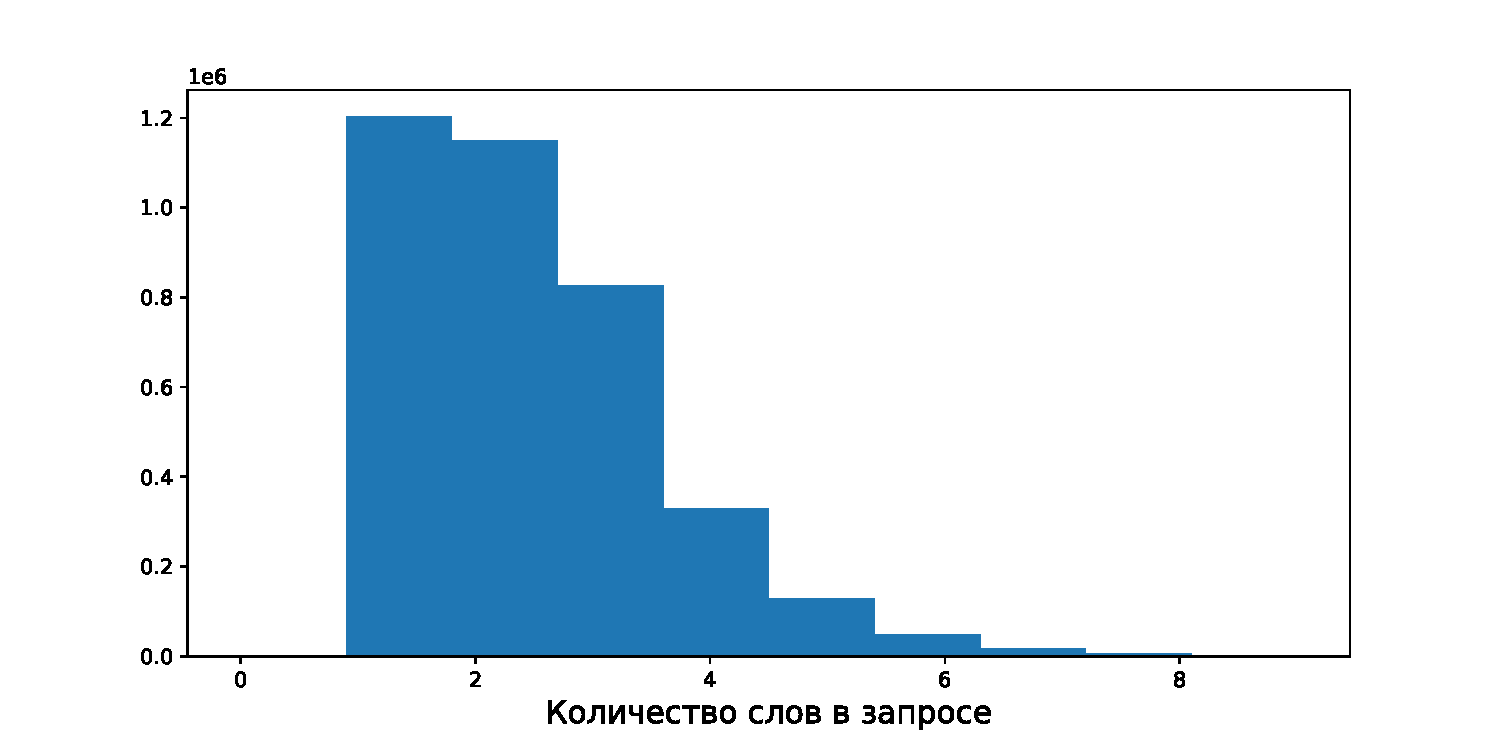
\includegraphics[scale=0.4]{nwords.pdf}
	\end{center}
	\caption{Распределение числа слов в запросе}
\end{figure}

\begin{figure}[H]
	\begin{center}
		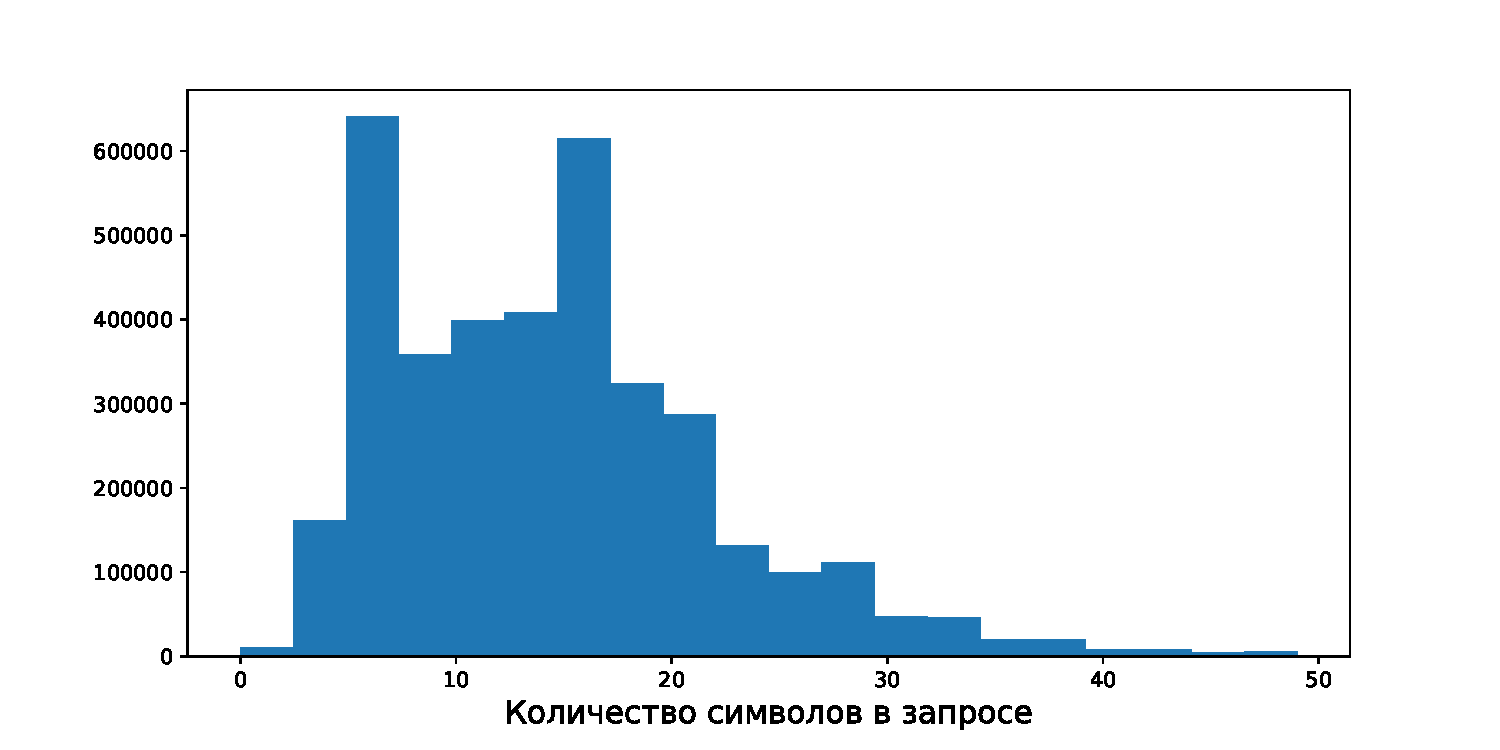
\includegraphics[scale=0.4]{nsym.pdf}
	\end{center}
	\caption{Распределение числа символов в запросе}
\end{figure}

\noindent Поскольку длины входных последовательностей невелики, мы можем уменьшить число головок внимания, так как их будет достаточно для того, чтобы модель смогла учитывать контекст. Кроме того, уменьшение числа параметров способствует более быстрому обучению и снижает эффект переобучения. После стадии предобучения, к модели также добавляет линейный слой и softmax слой для дообучения на непосредственно распознавание именованных сущностей. Полученная модель имеет порядка 66 млн. параметров.

В качестве токенизатора будем использовать ставший для BERT классическим WordPiece\cite{wordpiece}. Данный алгоритм токенизации разбивает входные слова на буквы, а затем, используя статистики по корпусу, начинает их сливать, до того момента, пока в словаре не окажется заранее выбранное число токенов. В итоге чаще всего многие слова оказываются разбитыми на более мелкие подслова (к примеру, слово \textit{токенизатор} может быть разбито на слова \textit{токен}, \textit{\#\#изатор}. В этом случае две решетки в начале подслова означают, что данный токен встречается внутри какого-то слова, но не является его началом). Данный подход (разбиение слов на более мелкие подслова) оказывается весьма полезным в контексте нашей задачи. Дело в том, что пользователи часто могут допустить опечатки в своем запросе. В случае, если бы токенизатор использовал все слово целиком в качестве самостоятельной единицы, чаще всего модель бы не нашла его в своем словаре. Однако когда в качестве токенов используются подслова, в случае ошибки, пользователь чаще всего ошибается лишь в одном из подслов, что позволяет модели относительно качественно отработать в данном случае.

  
\section{Обучение модели}

\subsection{Токенизатор}

В описанной в предыдущих разделах статье \cite{ner} было установлено, что стандартные предобученные токенизаторы в рамках рассматриваемой задачи покрывают достаточно малое количество токенов:

\begin{figure}[H]
	\begin{center}
		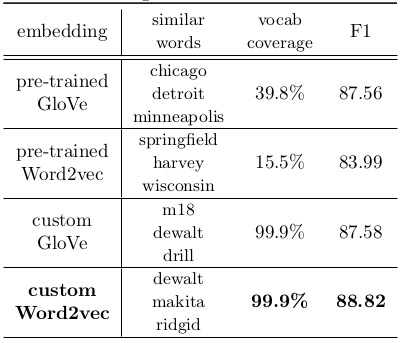
\includegraphics[scale=0.4]{tab2.jpg}
	\end{center}
	\caption{Покрытие словаря различными токенизаторами \cite{ner}}
\end{figure}

\noindent Как видно из таблицы, предобученные эмбеддинги покрывают лишь порядка 15-40\% встречающихся токенов. Этот факт, а также мотивация из предыдущего раздела (про опечатки) спродвигли автора на обучение собственного токенизатора WordPiece. Токенизатор обучался на всех имеющихся данных, его итоговый размер составил 30.000 токенов.

\subsection{Предобучение.}

Предобучение проводилось на задаче предсказания маскированных слов (MLM). В качестве обучающего датасета использовалась база названий товаров, составленная из нескольких компонент, описанных в соответствующем разделе. После препроцессинга и удаления дубликатов размер набора данных составил 3.268.226 сэмплов. Из них 10.000 примеров были отложены в качестве валидационной выборки. Обучение велось в течение 12 часов на графическом процессоре NVIDIA RTX 3090. За это время модель прошла около 8 эпох. Функция ошибки (кросс-энтропия) на обучающем и валидационном наборах данных представлена на рисунке 14. Как видно, большой размер обучающих данных позволил модели стабильно уменьшать значения функции ошибки как на обучающем датасете, так и на валидации. При этом графики выходят на некоторое плато, дальнейшее обучение несущественно влияет на качество полученной нейросети.

\begin{figure}[H]
	\begin{center}
		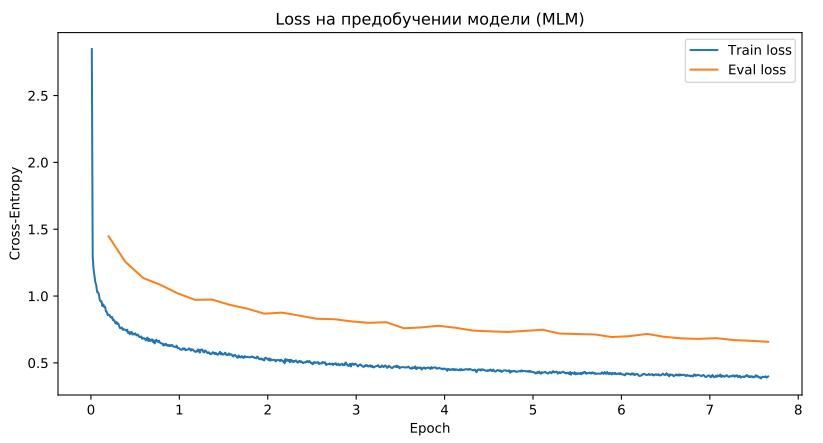
\includegraphics[scale=0.4]{loss_pretrain.jpg}
	\end{center}
	\caption{Функция ошибки на этапе предобучения}
\end{figure}

\noindent 

\subsection{Дообучение.}

Дообучение проводилось на размеченных людьми данных. В качестве обучающей выборки было выделено 9500 сэмплов, оставшиеся 500 были отложены для валидации. Во время проведения экспериментов было обнаружено, что такого количества примеров недостаточно для стабильного обучения модели в течение большого количества эпох. В связи с этим в процесс обучения были внесены поправки: вероятность dropout была увеличена до 0.2 (в оригинальном BERT - 0.1), коэффициент L2-регуляризации (в контексте нейросетей известный как Weight Decay) был увеличен до 0.1 (был 0.0). Эти модификации позволили относительно успешно тренировать модель на протяжении трех эпох.

\begin{figure}[H]
	\begin{center}
		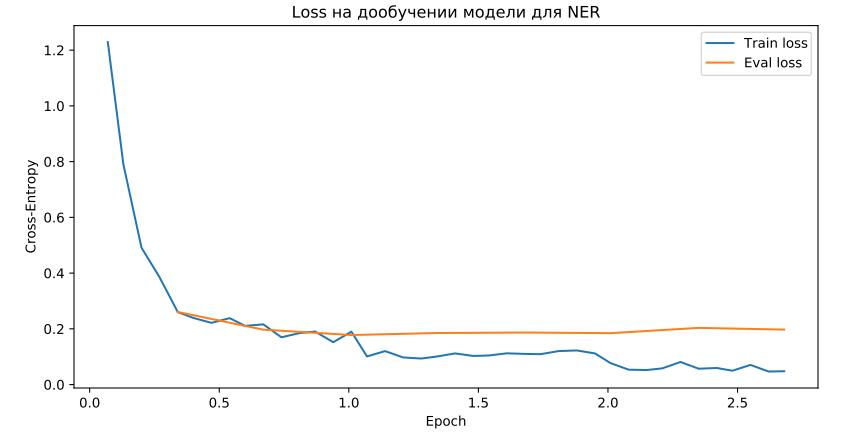
\includegraphics[scale=0.4]{loss_ner.jpg}
	\end{center}
	\caption{Функция ошибки на этапе NER}
\end{figure}

\noindent Как можно заметить, качество на валидации к концу первой эпохи выходит на минимум. Далее уменьшается лишь качество на обучающей выборке. Если продолжить тренировать модель, то начнется переобучение (качество на обучении будет повышаться, а на валидации - падать). Это происходит из-за того, что обучающая выборка достаточно мала, поскольку данное исследование является некоммерческим, а разметка большого количества запросов является финансово затратной процедурой.

\section{Результаты и примеры работы моделей}

В результате обучения описанных в предыдущем разделе моделей, были получены 2 предобученные нейросети: BERT для предсказывания замаскированных слов, а также BERT для распознавания именованных сущностей. В таблице 7 представлена матрица ошибок (confusion matrix) для полученной модели NER на валидационной выборке. Используемые обозначения: \textbf{r} --- истинная (real) метка слова, \textbf{p} --- предсказанная (predicted) моделью метка. Значения меток: \textbf{O} --- отсутствие класса, \textbf{I} --- название товара, \textbf{B} --- название бренда. Итоговая точность (accuracy) работы NER-сети составила \textbf{0.939}, а F1-мера \textbf{0.912}. Полученные результаты сложно сопоставлять со значениями метрик качества моделей, полученных в \cite{ner}, поскольку в данной работе размер валидационный выборки (500 сэмплов) был существенно меньше, чем в работе исследователей из TheHomeDepot (16915 сэмплов).

\begin{table}[H]
    \begin{center}
    \scalebox{1.0}{
    \begin{tabular}{ | c | c | c | c | } 
    \hline
     & \textbf{p = O} & \textbf{p = I} & \textbf{p = B} \\ 
    \hline
    \textbf{r = O} & 654 & 20 & 7 \\ 
    \hline
    \textbf{r = I} & 22 & 412 & 6 \\ 
    \hline
    \textbf{r = B} & 9 & 6 & 13 \\ 
    \hline
    \end{tabular}}
    \caption{Матрица ошибок для NER на валидационной выборке}
    \end{center}
\end{table}

\noindent Ниже представлены примеры работы обученных NER и MLM сетей.

\begin{figure}[H]
	\begin{center}
		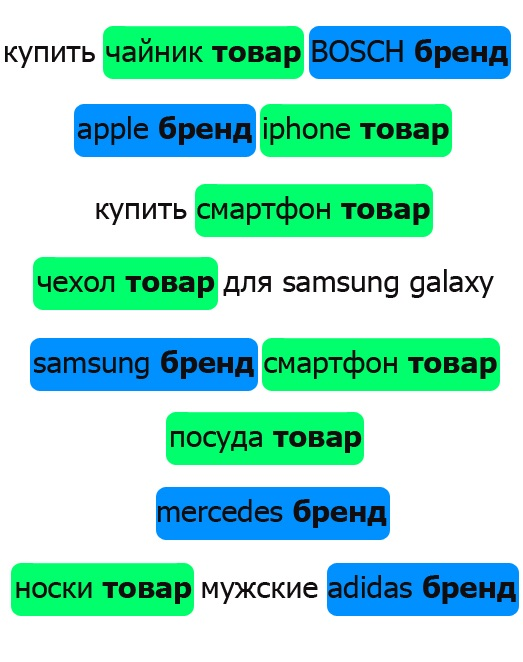
\includegraphics[scale=0.5]{ner2.jpg}
	\end{center}
	\caption{Примеры распознавания именованных сущностей.}
\end{figure}

\noindent Можно заметить, как модель использует контекст: в 4-м примере Samsung является брендом телефона, для которого покупается чехол, а не самим брендом чехла, поэтому данное слово не классифицируется как бренд. А в 5-м, наоборот, Samsung является брендом желаемого смартфона.

\begin{table}[H]
\begin{center}
\scalebox{0.8}{
\begin{tabular}{ |c|c|c|c| } 
\hline
Вход нейросети & Предложенный вариант & Вероятность \\
\hline
\multirow{2}{19em}{чехол для [MASK] galaxy} & чехол для samsung galaxy & 0.554 \\ 
& чехол для телефона galaxy & 0.061 \\ 
\hline

\multirow{3}{19em}{купить [MASK] для iphone 6} & купить чехол для iphone 6 & 0.961 \\ 
& купить стекло для iphone 6 & 0.003 \\ 
& купить наклеики для iphone 6 & 0.003 \\ 
\hline

\multirow{1}{19em}{купить [MASK] bosch 2 литра} & купить чаиник bosch 2 литра & 0.074 \\ 
\hline

\multirow{4}{19em}{молоко [MASK] ультрапастеризованное} & молоко питьевое ультрапастеризованное & 0.129 \\ 
& молоко фрутоняня ультрапастеризованное & 0.046 \\ 
& молоко свитлогорье ультрапастеризованное & 0.043 \\ 
& молоко вкуснотеево ультрапастеризованное & 0.029 \\ 
\hline
\end{tabular}}
\caption{Примеры предсказаний замаскированных слов.}
\end{center}
\end{table}

\noindent Помимо использования модели MLM в качестве базовой модели, которая будет дообучаться для NER, в контексте рассматриваемой задачи её также можно использовать для предложения следующего слова в запросе пользователя. Для этого необходимо указывать в качестве маскируемого слова последний (виртуальный) токен, после уже написанного пользователем куска запроса.

\begin{table}[H]
\begin{center}
\scalebox{1.0}{
\begin{tabular}{ |c|c|c|c| } 
\hline
Вход нейросети & Предложенный вариант & Вероятность \\
\hline
\multirow{3}{14em}{iphone [MASK]} & iphone 7 & 0.020 \\ 
& iphone 6 & 0.019 \\ 
& iphone 4 & 0.018 \\ 
\hline

\multirow{3}{14em}{купить яблоки [MASK]} & купить яблоки вес & 0.089 \\ 
& купить яблоки кг & 0.054 \\ 
& купить яблоки зеленые & 0.033 \\ 
\hline

\multirow{3}{14em}{смартфон samsung [MASK]} & смартфон samsung galaxy & 0.074 \\ 
& смартфон samsung note & 0.050 \\ 
& смартфон samsung s & 0.040 \\ 
\hline
\end{tabular}}
\caption{Предложение следующего слова при вводе пользователем запроса.}
\end{center}
\end{table}

\section{Заключение}
В качестве основных результатов данного исследования:
\begin{itemize}
    \item Рассмотрена задача построение поисковой системы для абстрактного интернет-магазина с использованием алгоритмов глубокого обучения
    \item Собран обучающий набор данных, часть из них была вручную размечена
    \item Проведен обзор релевантных данной тематике статей и подходов
    \item Предложена нейросетевая архитектура, основанная на BERT, для решения поставленной задачи
    \item Построены прототипы моделей, решающих поставленные задачи, представлены соответствующие им графики и метрики качества работы
\end{itemize}

\noindent В ходе работы были также получены дополнительные (бонусные) результаты:
\begin{itemize}
    \item Указаны ключевые сложности со сбором данных, которые возникнут у гипотетического исследователя, который захочет заниматься данной областью 
    \item Предложен метод сбора запросов пользователей в интернет-магазины через посредников --- общие поисковые системы (Яндекс, Google и т.д.)
    \item Предложен метод токенизации входных запросов, который способствует более качественной работе модели в случае, когда пользователь допустил опечатку в запросе
    \item Предложен метод предсказания следующего слова в запросе пользователя с помощью BERT, обученного на задачу MLM
\end{itemize}

Безусловно, построенные модели являются лишь прототипами. Для внедрения их в реальные бизнес-процессы потребуется дополнительная работа. В частности, для повышения качества работы необходимо будет разметить больший набор запросов, а также дополнить обучающий датасет синтетическими данными, как это было описано в \cite{ner}.

\section{Приложение}

Весь код для препроцессинга входных данных, предобучения модели, дообучения и выполнения предсказаний можно найти на GitHub репозитории автора: \href{https://github.com/Sorrow321/cmc\_seminar/}

Помимо этого, по указанной ссылке можно найти обученные в ходе работы модели, что позволит читателю самостоятельно провести интересующие его дополнительные эксперименты, а также убедиться в полученных результатах.

\section{Благодарности}
Автор выражает благодарность компании KazanExpress и, в частности, Юрию Гаврилину, за выделенные на безвозмездной основе данные --- запросы в поискую систему их интернет-магазина. 

Автор выражает благодарность компании LabelMe за льготные условия при выполнении разметки 10.000 запросов.

\bibliography{bibliography} 
\bibliographystyle{plain}

\end{document}
